\section{The Orchestration Framework}
\label{sec:framework}

The framework has four parts: a vocabulary of roles, a rule that sets each task's
autonomy, a protocol by which work passes between agents, and a model of the researcher's
review attention that bounds the size of the team. Figure~\ref{fig:overview} shows how
the parts fit together. The material condenses Chapters 1, 9, 10 and 17 of the source
textbook~\cite{mccreary2026aiforee}; the formal statements, the monotonicity result, the
derived planning-to-execution ratio, the sampling and escape terms of the attention model,
and the provenance rule are this paper's additions.

\begin{figure}[htbp]
  \centering
  % Figure: overview of the orchestration framework (Section 4).
\definecolor{oiblue}{HTML}{0072B2}
\definecolor{oiorange}{HTML}{E69F00}
\definecolor{oigreen}{HTML}{009E73}
\definecolor{oipurple}{HTML}{CC79A7}
\begin{tikzpicture}[
    font=\footnotesize,
    box/.style={draw, rounded corners=2pt, align=center, minimum height=11mm, inner sep=3pt},
    arrow/.style={-{Latex[length=2mm]}, thick},
    lab/.style={font=\scriptsize, align=center, fill=white, inner sep=1pt}]
  \node[box, fill=gray!12, text width=80mm] (R)
    {\textbf{Researcher (orchestrator)}\\question and acceptance criteria $\cdot$ gates\\
     acceptance of claims $\cdot$ daily review budget $B$};
  \node[box, fill=oigreen!10, text width=50mm, below=17mm of R] (W)
    {\textbf{Shared workspace} (version-controlled files)\\each artifact carries a status:\\
     \textsf{queued} $\rightarrow$ \textsf{running} $\rightarrow$ \textsf{needs-review}\\
     $\rightarrow$ \textsf{accepted} / \textsf{rejected}};
  \node[box, fill=oiblue!10, text width=25mm, left=17mm of W] (P)
    {\textbf{Planning agents}\\($n_p$): survey,\\decompose, specify};
  \node[box, fill=oiorange!15, text width=25mm, right=19mm of W] (E)
    {\textbf{Execution agents}\\($n_e$): code,\\analysis,\\figures, text};
  \node[box, fill=oipurple!12, text width=50mm, below=11mm of W] (C)
    {\textbf{Checks}: tests, validators, strict build, reviewer agent};
  \draw[arrow] (R.west) -| node[lab, pos=0.78]{question,\\constraints} (P.north);
  \draw[arrow] (P.east) -- node[lab, above=1pt]{plans,\\specs} (W.west);
  \draw[arrow] ([yshift=2.5mm]W.east) -- node[lab, above=1pt]{tasks} ([yshift=2.5mm]E.west);
  \draw[arrow] ([yshift=-2.5mm]E.west) -- node[lab, below=1pt]{artifacts,\\checks run} ([yshift=-2.5mm]W.east);
  \draw[arrow] ([xshift=-9mm]W.south) -- node[lab, left=1pt]{needs-review} ([xshift=-9mm]C.north);
  \draw[arrow] ([xshift=9mm]C.north) -- node[lab, right=1pt]{pass / defects} ([xshift=9mm]W.south);
  \draw[arrow, very thick, densely dashed] (W.north) -- node[lab, right=2pt]{gate: claims, irreversible\\or outward-bound actions} (R.south);
  \draw[arrow] (R.east) -| node[lab, pos=0.78]{approve\\level-1 steps} (E.north);
\end{tikzpicture}

  \caption{The orchestration framework. Planning agents turn the researcher's question
  into plans and specifications; execution agents turn specifications into artifacts.
  All work passes through a shared, version-controlled workspace in which each artifact
  carries a status. Scripts and reviewer agents check artifacts, but only the researcher
  accepts claims and approves irreversible or outward-bound actions. Note that the
  researcher's daily review budget $B$, not the number of agents, sets the team size.}
  \label{fig:overview}
\end{figure}

\subsection{Definitions}
\label{sec:definitions}

\begin{description}[leftmargin=1.2em,style=nextline]
  \item[Research workflow] The sequence of repeatable activities by which a research
    question becomes a validated, communicated result: literature search, problem
    framing, scientific coding, data analysis and manuscript preparation, chained so that
    the output of each is the input of the next.
  \item[Task and artifact] A task is a unit of delegated work with a stated input, a
    bounded scope, an inspectable output (the \textit{artifact}) and an acceptance check
    that can pass or fail without redoing the work.
  \item[Agent] A system that uses a language model to choose actions, invokes tools to
    take them, observes the results and repeats until a goal is met or it stops to
    ask~\cite{yao2023react}. An \textit{assistant} differs in that the human takes every
    action in the world.
  \item[Orchestrator] Whoever decides what is done, by which agent, in what order, with
    what checks, and what happens on failure. Here the orchestrator is the researcher,
    who may be helped by an agent that keeps the task queue and drafts status reports but
    remains accountable for the result.
  \item[Check, gate and acceptance] A \textit{check} examines an artifact against its
    acceptance criteria; it may be mechanical (a test, a validator, a strict build) or
    performed by a reviewer agent. A \textit{gate} is a check at which the researcher
    must approve before work continues. \textit{Acceptance} is the decision that an
    artifact meets its criteria and may be used downstream.
\end{description}

\subsection{Roles}
\label{sec:roles}

Each agent holds one role, written once as a specification file and reused. One role
per agent has the same benefits as single-purpose software modules: a short instruction
set, a checkable output and failures that localize. Table~\ref{tab:roles} lists the
roles. The two primary roles differ in the cost of their output. A planning agent
surveys, decomposes and specifies; its output is a document that is cheap to read and
cheap to discard. An execution agent writes code, runs analyses and prepares figures and
text; its output changes files and consumes compute, and each unit costs more attention
to check. The \textit{planner--executor pattern} makes the specification the handoff
between them, so that a plan can be corrected before anything is
executed~\cite{shen2023hugginggpt,wang2023planandsolve,schluntz2024building}.
A reviewer agent checks another agent's output against stated criteria; because model
judges share the biases of models~\cite{zheng2023judging}, it complements mechanical
checks and the researcher's sampling rather than replacing them. Each agent receives
only the context its role needs (\textit{context isolation}), which limits distraction
in long contexts~\cite{liu2024lost} and limits what an agent that reads untrusted
content can leak or be steered into~\cite{greshake2023injection}.

\begin{table}[htbp]
  \centering
  \caption{Agent roles with their usual artifact, default autonomy ceiling (levels
  defined in Table~\ref{tab:levels}) and the check applied before acceptance. Domain
  roles specialize a planning or execution role.}
  \label{tab:roles}
  \small
  \begin{tabular}{L{2.6cm}L{4.3cm}L{2.9cm}C{1.3cm}L{3.0cm}}
    \toprule
    Role & Purpose & Artifact & Level & Check \\
    \midrule
    Planning & Survey, decompose, specify & Plan, specification & 2--3 & Researcher reads plan \\
    Execution & Carry out a specified task & Files, results & 1--2 & Acceptance criteria, tests \\
    Reviewer & Check output against criteria & Defect list & 3 & Sample of its findings \\
    \midrule
    Literature & Search, triage, extract claims & Reading list with claim locations & 2 & Citation lookup \\
    Analysis & Run statistical and signal processing & Tables, plots & 2 & Known-answer tests \\
    Coding & Write and test code & Scripts, tests & 2 & Tests, diff review \\
    Writing & Draft prose from claims & Section drafts & 2 & Claim audit by researcher \\
    \bottomrule
  \end{tabular}
\end{table}

\subsection{Autonomy levels and the assignment rule}
\label{sec:autonomy}

Autonomy is the degree to which an agent acts without a human decision at each step.
The framework uses four levels (Table~\ref{tab:levels}). Following the principle that
automation should be chosen by the consequences of actions~\cite{parasuraman2000model},
the level is set from three Boolean properties of a task's \emph{effects}, not from
confidence in the model:
\begin{itemize}[leftmargin=*]
  \item \textit{Reach} $X(t)$: the result leaves the researcher's control---it is sent,
    published, written to a shared system or commits resources ($X=1$).
  \item \textit{Reversibility} $R(t)$: the effect can be undone, as a change to a
    version-controlled file can and a sent message cannot ($R=1$).
  \item \textit{Verifiability} $V(t)$: the result can be checked quickly and
    objectively, by a script or a short human inspection ($V=1$); a program with tests is
    verifiable, a paragraph of related work is not without reading the cited papers.
\end{itemize}

\begin{table}[htbp]
  \centering
  \caption{Autonomy levels. The level is a ceiling for the task; an agent operates at or
  below it, and only after evaluation shows that it performs the task reliably.}
  \label{tab:levels}
  \small
  \begin{tabular}{C{0.9cm}L{3.0cm}L{5.0cm}L{5.2cm}}
    \toprule
    Level & Name & The agent may & Typical use \\
    \midrule
    0 & Suggest only & Propose; the researcher performs the action & Outward-bound results that cannot be verified \\
    1 & Approve each step & Act after each action is approved & Irreversible, or outward-bound but verifiable \\
    2 & Act within a boundary & Act inside a defined scope; stop at gates & Local, reversible work whose quality needs a human read \\
    3 & Act and report & Act unattended; report afterwards & Local, reversible, mechanically verifiable work \\
    \bottomrule
  \end{tabular}
\end{table}

The assignment rule, shown as a decision tree in Figure~\ref{fig:autonomy}, maps the three
properties to a level:
\begin{equation}
  \lambda(t) =
  \begin{cases}
    0 & \text{if } X=1 \text{ and } V=0,\\
    1 & \text{if } X=1 \text{ and } V=1, \text{ or } X=0 \text{ and } R=0,\\
    2 & \text{if } X=0,\ R=1 \text{ and } V=0,\\
    3 & \text{if } X=0,\ R=1 \text{ and } V=1.
  \end{cases}
  \label{eq:rule}
\end{equation}

\begin{figure}[htbp]
  \centering
  % Figure: the autonomy assignment rule, Equation (1), as a decision tree read left to right
% (Section 4.3).
\definecolor{oiblue}{HTML}{0072B2}
\definecolor{oivermillion}{HTML}{D55E00}
\begin{tikzpicture}[
    font=\footnotesize,
    q/.style={draw, rounded corners=2pt, align=center, fill=gray!10, text width=25mm, minimum height=9mm, inner sep=2pt},
    leaf/.style={draw, align=center, text width=24mm, minimum height=8.5mm, inner sep=2pt},
    arrow/.style={-{Latex[length=2mm]}, thick},
    yes/.style={font=\scriptsize, fill=white, inner sep=1pt}]
  \node[q] (X) at (0, 0) {Result leaves your control? (reach $X$)};
  \node[q] (V1) at (3.9, 1.6) {Verifiable? ($V$)};
  \node[q] (Rv) at (3.9, -1.3) {Reversible? ($R$)};
  \node[leaf, fill=oivermillion!22] (L0) at (8.0, 2.3) {\textbf{Level 0}\\Suggest only};
  \node[leaf, fill=oivermillion!8] (L1a) at (8.0, 0.95) {\textbf{Level 1}\\Approve each step};
  \node[leaf, fill=oivermillion!8] (L1b) at (8.0, -0.4) {\textbf{Level 1}\\Approve each step};
  \node[q] (V2) at (8.0, -2.2) {Verifiable? ($V$)};
  \node[leaf, fill=oiblue!8] (L2) at (12.1, -1.55) {\textbf{Level 2}\\Act within boundary};
  \node[leaf, fill=oiblue!22] (L3) at (12.1, -2.85) {\textbf{Level 3}\\Act and report};
  \draw[arrow] (X.east) -- node[yes]{yes} (V1.west);
  \draw[arrow] (X.east) -- node[yes]{no} (Rv.west);
  \draw[arrow] (V1.east) -- node[yes]{no} (L0.west);
  \draw[arrow] (V1.east) -- node[yes]{yes} (L1a.west);
  \draw[arrow] (Rv.east) -- node[yes]{no} (L1b.west);
  \draw[arrow] (Rv.east) -- node[yes]{yes} (V2.west);
  \draw[arrow] (V2.east) -- node[yes]{no} (L2.west);
  \draw[arrow] (V2.east) -- node[yes]{yes} (L3.west);
\end{tikzpicture}

  \caption{The autonomy assignment rule of Equation~\eqref{eq:rule} as a decision tree.
  Reach is tested first because an outward-bound result cannot be recalled, whatever
  its other properties. Note that an irreversible local action receives level 1 even when
  it is verifiable, since a check after the fact cannot undo it.}
  \label{fig:autonomy}
\end{figure}

\paragraph{Proposition 1 (completeness and monotonicity).} \textit{The rule assigns
exactly one level to each of the eight combinations of $(X,R,V)$, and making a task safer
in any one property---$X$ from 1 to 0, $R$ from 0 to 1, or $V$ from 0 to 1---never lowers
its level.}

\textit{Proof.} The four cases partition the space: $X=1$ is split by $V$, and $X=0$ is
split by $R$ and then, for $R=1$, by $V$. For monotonicity, consider each property in
turn. Raising $V$ moves $(X{=}1)$ from 0 to 1, leaves $(X{=}0,R{=}0)$ at 1, and moves
$(X{=}0,R{=}1)$ from 2 to 3. Raising $R$ leaves $X=1$ tasks unchanged and moves $X=0$
tasks from 1 to 2 or 3. Lowering $X$ moves $(V{=}0)$ tasks from 0 to 1 or 2 and $(V{=}1)$
tasks from 1 to 1 or 3. No transition decreases the level. $\square$

Monotonicity matters in practice because the cheapest way to raise an agent's autonomy is
to change the task, not the model: writing outputs to a new file instead of overwriting
raw data makes an action reversible, and adding a known-answer test makes it verifiable.
The level is a \emph{ceiling}. An agent operates at $\min(\lambda(t), \ell_e)$, where
$\ell_e$ is the level its evaluation on representative tasks supports; the evaluation is
repeated whenever the model, tools or instructions change.

\subsection{Failure modes and controls}
\label{sec:failures}

Agents fail in recognizable ways, and each failure leaves a signature in a log.
Table~\ref{tab:failures} lists six modes with the mechanical defense the framework
prescribes for each; they correspond to the system-design and task-verification
failures observed in multi-agent traces~\cite{cemri2025multiagent} and to test
exploitation by coding agents~\cite{zhong2025impossiblebench}. Logging is therefore a
precondition of autonomy above level 1: for each step the log records the time, the
tool and its arguments, the files changed, the model and its settings, and the result,
as activity logging proposals for agents recommend~\cite{chan2024visibility}.

\begin{table}[htbp]
  \centering
  \caption{Agent failure modes, how each appears in a log, and the mechanical defense
  that removes the need to catch it by careful reading.}
  \label{tab:failures}
  \small
  \begin{tabular}{L{3.0cm}L{5.4cm}L{5.8cm}}
    \toprule
    Failure mode & Log signature & Mechanical defense \\
    \midrule
    Premature completion & ``Done'' reported with no check output & Require the check output in the handoff \\
    Hallucinated result & A reported number with no producing tool call & Provenance rule: trace every number to a call \\
    Scope drift & Edits to files outside the task & Path permissions; diff review \\
    Test weakening & Test files changed alongside failing code & Protect tests; review test diffs first \\
    Wrong arguments & Tool errors, or results from the wrong file & Read the first calls of a new workflow \\
    Runaway loop & The same call repeated without progress & Step, time and spending limits; repeat detector \\
    \bottomrule
  \end{tabular}
\end{table}

\subsection{Handoff protocol and provenance}
\label{sec:handoff}

Work passes between agents as files in a shared, version-controlled workspace. Each
agent writes to its own directory or branch, inputs are read-only, and merging is a
reviewed step. Every artifact carries a status from the set
$S=\{\textsf{queued},\textsf{running},\textsf{needs-review},\textsf{accepted},\textsf{rejected}\}$,
with transitions $\textsf{queued}\rightarrow\textsf{running}\rightarrow\textsf{needs-review}
\rightarrow\{\textsf{accepted},\textsf{rejected}\}$ and $\textsf{rejected}\rightarrow\textsf{queued}$.
The protocol imposes three invariants and one rule:
\begin{enumerate}[leftmargin=*,label=\textbf{I\arabic*}]
  \item \textit{Separation of acceptance.} For every artifact $a$,
    $\mathrm{acceptor}(a)\neq\mathrm{producer}(a)$: no agent sets \textsf{accepted} on its
    own output. A script, a reviewer agent or the researcher may.
  \item \textit{Level-bounded acceptors.} Artifacts of level-3 tasks may be accepted by a
    script; artifacts of level-0 and level-1 tasks are accepted only by the researcher.
  \item \textit{Claim gate.} Any artifact whose content becomes a reported
    claim---a number, a citation or a conclusion in a manuscript---is accepted only by the
    researcher, whatever the level of the task that produced it.
  \item[\textbf{P}] \textit{Provenance.} Every number that an agent reports as computed
    names the command or script and the input that produced it. A number without a
    producing call is treated as unverified and blocks acceptance.
\end{enumerate}
The provenance rule was added after the case analysis of Section~\ref{sec:cross-case}
showed a defect that no other control could catch. A handoff record that satisfies the
protocol fits in a few lines (Listing~1).

\begin{lstlisting}[caption={An illustrative handoff record for the ENOB analysis script of
Section~\ref{sec:case-a}, written as YAML at the top of the artifact.}]
task: T3-enob-script          # from the task queue
role: coding-agent            # producer
level: 3                      # ceiling from Eq. (1): local, reversible, verifiable
status: needs-review          # producer may not set "accepted" (I1)
inputs: [docs/procedure.md@a1c3f2, data/ideal-10bit.csv]
outputs: [scripts/enob.py]    # the only path it may write
acceptance:
  - known-answer: ideal 10-bit record gives SNDR 61.96 dB (+/- 0.05)
  - boundary: empty or wrong-length record raises an error
check_output: logs/T3-check.txt
numbers:                       # provenance rule P
  - {value: "61.96 dB", source: "logs/T3-check.txt:14"}
open_questions: [window choice for non-coherent records]
\end{lstlisting}

\subsection{Attention budget and span of control}
\label{sec:attention}

Let a team have $n_p$ planning and $n_e$ execution agents. An agent of class
$j\in\{p,e\}$ delivers $k_j$ artifacts per day; reading one takes the researcher $r_j$
minutes; the researcher reads a fraction $s_j\in(0,1]$ of them; and conflict resolution
and status reports take $c$ minutes a day. The daily review load is
\begin{equation}
  L = n_p k_p r_p s_p + n_e k_e r_e s_e + c ,
  \label{eq:load}
\end{equation}
and the team is feasible when $L\leq B$, the researcher's daily attention budget. For a
team of one class the \textit{span of control} is
\begin{equation}
  n_j^{\max} = \left\lfloor \frac{B-c}{k_j\, r_j\, s_j} \right\rfloor .
  \label{eq:span}
\end{equation}
Equation~\eqref{eq:span} plays the role of fan-out in supervisory
control~\cite{crandall2005validating,cummings2008predicting}: an agent that delivers an
artifact every $1/k_j$ days and needs $r_j s_j$ minutes of attention for each can be
neglected for the rest of the time. The difference is that the attention is spent on
verification after the fact rather than on control during the task.

The book's worked example uses illustrative values: $n_p=20$ and $n_e=10$, one artifact
per agent per day, $r_p=6$ and $r_e=15$ minutes, $s_p=s_e=1$ and $c=30$ minutes. Then
$L=120+150+30=300$ minutes. With a budget of four hours ($B=240$), the team is infeasible;
reading half of the planning artifacts ($s_p=0.5$) gives $L=60+150+30=240$ and restores
feasibility. Figure~\ref{fig:load} shows the load as the team grows under three review
regimes.

\begin{figure}[htbp]
  \centering
  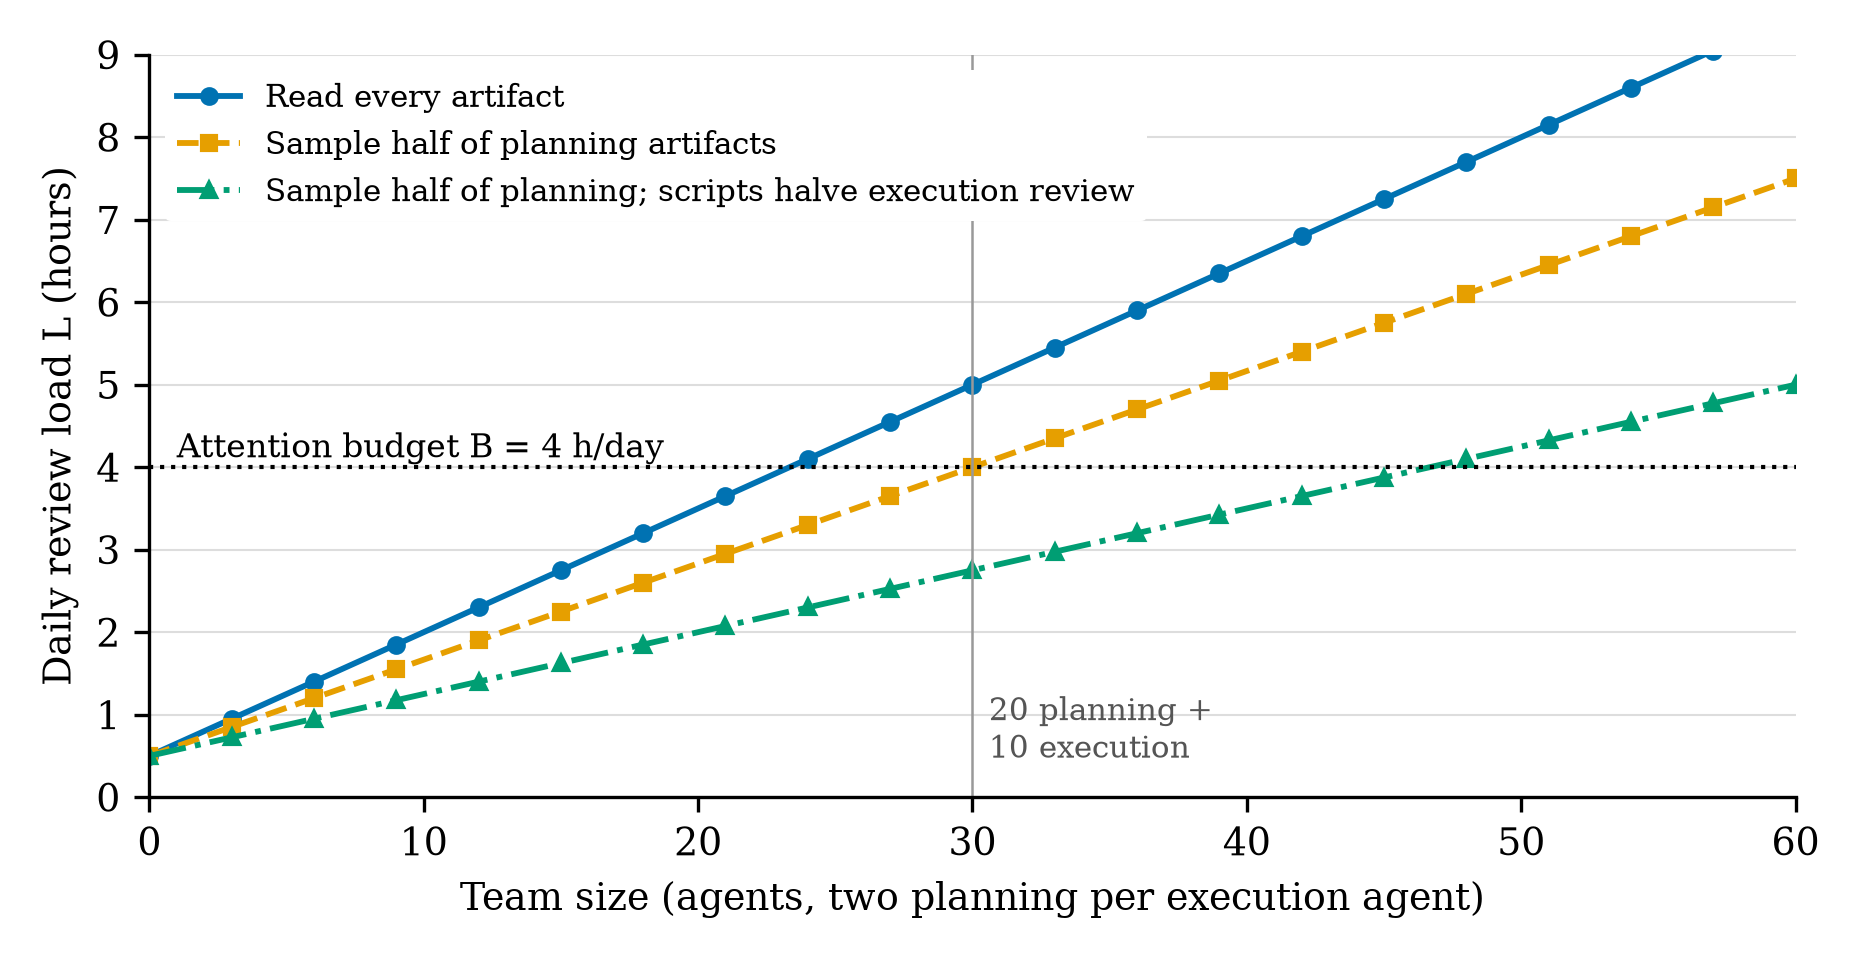
\includegraphics[width=0.85\textwidth]{figures/review-load.png}
  \caption{Daily review load $L$ (Equation~\ref{eq:load}) against team size for a team
  with two planning agents per execution agent, under three review regimes, with a
  four-hour attention budget. Parameters are the illustrative values of
  Section~\ref{sec:attention}, not measurements. Note that sampling planning output and
  replacing part of execution review with scripted checks each widen the span of
  control more than any change in the number of agents can.}
  \label{fig:load}
\end{figure}

\paragraph{The planning-to-execution ratio is derived, not fixed.} Suppose the researcher
gives a share $\beta$ of the net budget $B-c$ to reviewing plans. Applying
Equation~\eqref{eq:load} to each class gives
\begin{equation}
  \frac{n_p}{n_e} = \frac{\beta}{1-\beta}\cdot\frac{k_e\, r_e\, s_e}{k_p\, r_p\, s_p}.
  \label{eq:ratio}
\end{equation}
With the illustrative costs and an equal split ($\beta=0.5$) the ratio is $15/6=2.5$; the
book's 20:10 team corresponds to $\beta=120/270\approx0.44$. The ratio is therefore a
consequence of the relative cost of reviewing plans and executions. A known-answer test
that halves $r_e$ doubles the number of execution agents the same budget supports.

\paragraph{Sampling trades load for escaped defects.} Let an artifact of class $j$
contain a consequential defect with probability $q_j$, let mechanical checks detect it
with probability $a_j$, and let the researcher detect it with probability $h_j$ when the
artifact is read. The expected number of defects per day that pass review undetected is
\begin{equation}
  E = \sum_{j\in\{p,e\}} n_j\, k_j\, q_j\,(1-a_j)\,(1-s_j h_j).
  \label{eq:escape}
\end{equation}
Lowering $s_j$ reduces $L$ linearly but raises $E$; raising $a_j$ lowers $E$ without any
cost in $L$. Automation bias lowers $h_j$ as the researcher grows used to correct
output~\cite{parasuraman2010complacency}, so the framework prefers mechanical checks to
reduced sampling, reserves sampling for reversible planning output, and requires
reviewers to state an expected value or check a random sample rather than approve by
habit. $E$ is observable as the number of defects found after acceptance, and together
with $L$ it is the quantity to measure before a team is enlarged.

\paragraph{Checks at handoffs dominate improvements to single stages.} For a chain of $m$
stages in which stage $i$ introduces a consequential defect with probability $p_i$ and
the check at its handoff catches it with probability $d_i$, the probability that the
final result is free of such defects is
\begin{equation}
  P_{\mathrm{clean}} = \prod_{i=1}^{m}\bigl(1 - p_i(1-d_i)\bigr).
  \label{eq:pipeline}
\end{equation}
With five stages and $p_i=0.1$ (illustrative), $P_{\mathrm{clean}}=0.9^5\approx0.59$ with
no checks. Making one stage almost perfect ($p=0.01$) raises it only to about $0.65$,
whereas a check catching 80\% of defects at every handoff raises it to
$0.98^5\approx0.90$.

\paragraph{Dependencies bound what parallelism can buy.} The makespan of a set of tasks
cannot be shorter than the longest chain of dependent tasks, the critical
path~\cite{kelley1959critical}, however many agents are available, and each added agent
adds handoffs and potential conflicts~\cite{brooks1995mythical}. A team should therefore
grow one role at a time, and stop when an added agent adds more review than it removes
work.

\subsection{Design rationale and rejected alternatives}
\label{sec:rationale}

Five design decisions distinguish the framework, each taken against a named
alternative.
\begin{enumerate}[leftmargin=*]
  \item \textit{Autonomy from task effects, not model capability.} Capability-based
    levels change with every model release and say nothing about whether a result can be
    recalled. Role-based levels~\cite{feng2025levels} describe the interaction but give no
    rule for a task; the rule of Equation~\eqref{eq:rule} supplies one and is compatible
    with them (roughly, level 0 corresponds to the user as operator, level 1 to the user
    as approver and level 3 to the user as observer).
  \item \textit{Files, not conversations, as handoffs.} Conversational
    coordination~\cite{wu2023autogen,qian2024chatdev} is flexible, but a conversation is
    hard to diff, review or resume a month later. Files in version control give every
    handoff an author, a timestamp and a reversible history, at the cost of more
    up-front structure.
  \item \textit{A human orchestrator, not an autonomous one.} Fully automated research
    pipelines~\cite{lu2024aiscientist,schmidgall2025agentlab} remove the bottleneck this
    paper models, but they also remove the accountable party that venues
    require~\cite{arxiv2025genai,thorp2023chatgpt}, and they cannot produce physical
    measurements. An orchestrating agent may keep the queue; it may not accept claims.
  \item \textit{Reviewer agents as complements.} A reviewer agent scales review but
    shares the failure modes of the models it
    reviews~\cite{zheng2023judging,sharma2023sycophancy}; it is used to decide where the
    researcher looks, not what is true.
  \item \textit{Risk-weighted sampling instead of reading everything.} Reading every
    artifact is infeasible beyond a small team (Figure~\ref{fig:load}) and invites
    habitual approval~\cite{goddard2012automation}. The framework samples only reversible
    planning output and keeps full review for claims and irreversible actions.
\end{enumerate}
